\documentclass{article}
\usepackage[legalpaper, textwidth=450pt]{geometry}
\usepackage{amsmath,amssymb}
\DeclareMathOperator{\E}{\mathbb{E}}
\usepackage[utf8]{inputenc}
\usepackage[english]{babel}
\usepackage{biblatex}
\addbibresource{novel.bib}
\usepackage{graphicx}
\usepackage{indentfirst}
\usepackage{physics}
\usepackage{refcheck}
\usepackage{units}
\usepackage{wrapfig}
\usepackage{subcaption}
\usepackage{booktabs}
\usepackage{multirow}
\usepackage{graphicx}
\setkeys{Gin}{width=.7\textwidth}
\graphicspath{ {./images/} }

\title{Newsvendor Problems: A New Way to Integrated Forecasting and Optimisation}

\author{Congzheng Liu\thanks{Department of Management Science,
Lancaster University, Lancaster LA1 4YX, UK.
Email: {\tt \{c.liu19,a.n.letchford,i.svetunkov\}@lancaster.ac.uk}}
\and Adam N.\ Letchford$^*$ \and Ivan Svetunkov$^*$} % end author list

\date{Draft, 16th May 2020}

\begin{document}

\maketitle

\begin{abstract}
Newsvendor problems form a classical and important family of stochastic optimisation problems. The standard solution approach decomposes the problem into two steps: estimation of the demand distribution, then determination of the optimal production quantity (or quantities) for the given distribution. We propose a new, integrated solution approach, which estimates the optimal production quantity directly from the data. Our approach can be used even when the demand distribution is not stationary. Some encouraging computational results are given. 
\\*[2mm]
{\bf Keywords:} newsvendor problems, forecasting, data-driven optimisation, sales and operations planning
\end{abstract}


%%%%%%%%%%%%%%%%%%%%%%%%%%%%%%
\section{Introduction}

Inventory control is a classical and important topic in Operations Research and Operations Management (see, e.g., the books \cite{Po02,SPP98,Zi00}). In this paper, we focus on \emph{Newsvendor Problem} (NVP), which referrs to a \emph{single-period} \emph{stochastic} inventory control problem.

In early works on NVP \cite{AHM51,MK51}, it is assumed that the demand in each time period comes from a known probability distribution. Of course, in practice, this is not the case --- a fact already noted in 1958 by Scarf \cite{Sc58}. Assuming that historical demand data is available, one can attempt to address this difficulty by decomposing the problem into an estimation / forecasting phase and an optimisation phase.
In the first phase, one makes some assumption (e.g., normality) regarding the underlying data generating process, and uses the past data to estimate the parameters of the process.
In the second phase, one determines the order quantity (or quantities) based on the estimated parameter values.

Throughout this paper, we will call this two-phase approach the \emph{disjoint} approach. An advantage of the disjoint approach is that forecasting and optimisation experts can operate independently within an organisation. This makes things easier to manage. On the other hand, as noticed by several authors \cite{BT06,BM12,Ka94,KT96,KTB20}, there are two disadvantages:
\begin{itemize}
\item The two phases use different objective functions. Indeed, in the first phase, the objective is to minimise a function of the forecasting errors, such as the root mean square error or mean absolute error. In the second phase, however, the goal is usually to maximise expected profit.
\item If the forecasting model is misspecified, and/or there is substantial noise in the data, the effect on the optimisation phase is very hard to predict. In particular, upside and downside errors may have very different effects on expected profit.
\end{itemize}

An alternative to the disjoint approach is to use a single, \textit{integrated} approach, in which the order quantities are determined directly from the data. A simple example of an integrated approach is \emph{quantile regression} \cite{Br16,Hu19}. A nice feature of quantile regression is that it makes no assumptions about the demand distribution. Unfortunately, it can only be applied to relatively simple NVPs, for which one can express the optimal order quantities in terms of quantiles of demand.

In this paper, we introduce a new integrated approach. It is very flexible, and can be applied to a wide variety of NVPs, with complex profit functions. Roughly speaking, it involves forecasting the optimal order quantities instead of the demand. Moreover, instead of determining parameter values that minimise some function of the forecasting errors, our approach attempts to maximise the expected profit directly.

After explaining our approach formally, we show that it reduces to quantile regression in the case of the simplest NVP (with only one product, stationary demand, and linear profit functions).  We then perform extensive computational experiments, on several different NVPs. The results show that our method performs well, in comparison with the disjoint approach, according to several different measures of quality.

The rest of the paper is organized as follows. Section \ref{se:lit} provides a brief review of the relevant literature. Section \ref{se:new} presents the new method and shows that it is a generalisation of quantile regression. In Section \ref{se:results}, we present and discuss the computational results. Finally, Section \ref{se:end} gives some insights, remarks and suggestions.

%%%%%%%%%%%%%%%%%%%%%%%%%%%%%%
\section{Literature Review} \label{se:lit}

Since the literature on NVPs is vast, we mention here only works of direct relevance. The reader looking for more information is directed to the books \cite{Ch12,Po02,SPP98,Zi00}.

\subsection{The classical newsvendor problem} %\label{sub:lit1}

In the simplest NVP, found in textbooks \cite{Ch12}, a company purchases goods at the beginning of a time period at a cost of $v$ per unit, and aims to sell them by the end of the period at a price $p$ per unit. The demand during the period is a random variable $Y$ with known probability density function $f$ and cumulative distribution function $F$. At the end of the period, any surplus goods will lead to a \emph{holding cost} of $c_h$ per unit. On the other hand, shortage of goods during the period will lead to a \emph{shortage cost} of $c_s$ per unit. The goal is to determine an \emph{order quantity} $Q$, prior to the period, that maximises the expected profit.

For a given $Q$ and a given realisation $y$ of $Y$, the profit over the period is:
\[
    \pi(Q,y)=
    \begin{cases}
        py-vQ-c_h(Q-y),& \text{if } Q\geq y\\
        pQ-vQ-c_s(y-Q),& \text{if } Q< y.
    \end{cases}
\]
The expected value of $\pi(Q,y)$ is:
\[
    \Pi(Q) = \int_{0}^{Q} \big[ py-vQ-c_h(Q-y) \big] f(y)dy + \int_{Q}^{\infty} \big[ pQ-vQ-c_s(y-Q) \big] f(y)dy.
\]

It is common to call $c_u= p-v+c_s$ the ‘underage’ cost and $c_o = v+c_h$ the ‘overage’ cost. Some calculus then shows that the order quantity that maximises $\Pi(Q)$ is:
\[
    Q^* = F^{-1}\left( \frac{c_u}{c_o+c_u} \right),
\]
where $F^{-1}$ is the inverse function of $F$. Thus, $Q^*$ is the $\tau$\textsuperscript{th} quantile of $f$, with $\tau=\nicefrac{c_u}{(c_o+c_u)}$.

\subsection{More complex newsvendor problems} %\label{sub:lit2}

Since the NVP was introduced in the 1950s \cite{AHM51,MK51}, researchers have considered several extensions of the problem, including variants with multiple product types \cite{HW63,LL96,MS00}, quantity discounts \cite{Kh95}, different risk measures \cite{EGS95}, product substitution \cite{BAA99}, nonlinear cost functions \cite{HOS12}, non-stationary demand \cite{KWH15}, and price setting \cite{KC62,Mi59,PD99}.

For the purpose of what follows, we now explain one variant, the `Nonlinear Newsvendor Problem' (NNVP), in detail (see also \cite{BT06,HOS12,HN16,KC62,Kh95,KK18,Mi59,PSC15,PD99}). In the NNVP, the profit function takes the form:
\[
    \pi(Q,y)=
    \begin{cases}
        P(Q,y)-V(Q)-C_h(Q,y),& \text{for } Q \geq y\\
        P(Q,y)-V(Q)-C_s(Q,y),& \text{for } Q< y,
    \end{cases}
\]
where $V$, $P$, $C_h$ and $C_s$ are now \emph{functions} rather than constants.

If $\pi(Q,y)$ has a particularly simple form (e.g., if it is piecewise-linear), then it may be possible to  use calculus to express the optimal order quantity as a quantile. In general, however, a closed-form expression as a quantile is unlikely to exist.

We now review one particular NNVP, taken from \cite{KK18,PD99,RK02}, that we are going to use in our numerical experiments. The purchase cost $v$ and selling price $p$ are constants, but $C_h$ and $C_s$ are functions. Overstock items incur a fixed unit penalty $\alpha > 0$, but they can be sold in a salvage market with fixed unit sales price $\beta$, with $0<\beta<v$. The demand in the salvage market is itself a random variable, with known distribution, which we denote by $u$. That is, we have:
\[
    C_h(Q,y) \, = \, \alpha[Q-y]^{+} - \beta \E \Big[ \min \big\{ [Q-y]^{+},u \big\} \Big].
\]
Moreover, the shortage penalty is proportional to the shortage quantity. That is:
\[
C_s(Q,y) =  \zeta \, \big( [y-Q]^{+} \big)^2
\]
for some constant $\zeta > 0$.

\subsection{Quantile regression} %\label{sub:lit3}

Returning to the classical NVP, we now consider the (more realistic) case in which the demand distribution is unknown, but we have historical demands $y_1,y_2,\dots,y_s$.
For this case, \emph{quantile regression}
has proven to perform rather well. The basic idea is as follows \cite{BT06,Br16,CS19,HNS15,Hu19}:
\begin{enumerate}
\item Compute the value of $\tau$ that maximises expected profit;
\item Use quantile regression to compute an estimate of the $\tau$\textsuperscript{th} quantile of the demand in the next time period, which we denote by $\hat{y}_{s+1}^{(\tau)}$;
\item Set the order quantity $\hat{Q}_{s+1}$ to $\hat{y}_{s+1}^{(\tau)}$.
\end{enumerate}

Unfortunately, quantile regression is efficient only on large samples \cite{Hu19,RV19}. Another drawback is that the performance of this approach depends crucially on the underlying target service level. In the experiments of Huber \cite{Hu19} and Rudin \cite{RV19}, the benefit of using the quantile regression method is limited to target service levels smaller than 0.8.

\subsection{Other integrated approaches} %\label{sub:lit4}

There exist other integrated methods. One approach is to use machine learning techniques, such as neural networks, to estimate the optimal order quantity from historical data. The application of machine learning to NVPs can be seen in \cite{CS19,OST20,RV19}. Another integrated approach is based on so-called \emph{one-shot decision theory} \cite{Guo11,GM14,Ma19}. A numerical example was shown in \cite{Guo11}, and extensions can be found in \cite{Ma19}. For the sake of brevity, we do not describe these alternative integrated methods in detail.

%%%%%%%%%%%%%%%%%%%%%%%%%%%%%
\section{The Proposed Estimator for NVPs} \label{se:new}

We have seen that, while quantile regression can be an attractive integrated approach, it has some drawbacks. In particular, for most non-trivial NVPs, it is very hard to express the optimal order quantity as a demand quantile \emph{a priori}. In order to overcome this limitation, we propose an alternative integrated method, based on a regression model with a specialised loss function.

For each historical period $t\in [1,s]$, we assume that the observed demand $y_t$ was a realisation of a random variable $Y_t$. Then, in principle, there exists an order quantity, say $Q_t^*$, that maximises the expected profit given $Y_t$ and $\Pi$. Thus, if we had set $Q_t$ to $Q_t^*$ prior to observing the true demand $y_t$, we would have maximised our expected profit in period $t$. Putting it another way, if we could somehow uncover the hidden structure of the time series $\big\{ Q_1^*,\dots,Q_s^* \big\}$, we would be able to estimate $Q_{s+1}^*$ directly.

Of course, in practice, the distributions $Y_t$ are unknown, and the values $Q_t^*$ are not observable. So we approximate the $Q_t^*$ values using a regression model. For each $t$, the regression model yields an estimate of $Q^*_t$, which we denote by $\hat{Q}_t$. The estimate $\hat{Q}_{s+1}$ can then be used as the order quantity in the next time period.

The crucial feature of our approach is that, instead of using the standard least-squares loss function to estimates the regression parameters, we choose the parameters that maximise the expected profit function $\sum_{t=1}^s{\pi \big( \hat{Q}_t,y_t \big)}$. In more detail, we modify the estimator of the model into:
\[
    \hat{\boldsymbol{\beta}}=\text{argmax}_{\boldsymbol{\beta}\in \mathbb{R}^{p+1}}\displaystyle\sum_{t=1}^s{\pi(\hat{Q}_t,y_t)},
\]
where we assume a linear relationship,
\[
    \mathbf{\hat{Q}}=\mathbf{X}\boldsymbol{\beta}
\]
and
\[
    \mathbf{\hat{Q}}=
    \begin{pmatrix}
        \hat{Q}_1\\
        \hat{Q}_2\\
        \vdots\\
        \hat{Q}_s
    \end{pmatrix},
    \mathbf{X}=
    \begin{pmatrix}
        \mathbf{x}_1^{\mathsf{T}}\\
        \mathbf{x}_2^{\mathsf{T}}\\
        \vdots\\
        \mathbf{x}_s^{\mathsf{T}}
    \end{pmatrix}=
    \begin{pmatrix}
        1&x_{11}&\cdots &x_{1p}\\
        1&x_{21}&\cdots &x_{2p}\\
        \vdots &\vdots &\ddots &\vdots \\
        1&x_{s1}&\cdots &x_{sp}
    \end{pmatrix},
    \boldsymbol{\beta}=
    \begin{pmatrix}
        \beta_0\\
        \beta_1\\
        \beta_2\\
        \vdots\\
        \beta_{p}
    \end{pmatrix},
\]
where where $\mathbf{x}_t^{\mathsf{T}}$ is the $t$th row of matrix $\mathbf{X}$, $p$ is the number of explanatory variables. While we focus on the linear regression model in this paper, the dynamic models, such as ARIMA or ETS \cite{HKO08}, can be used instead as efficiently. After estimating the model based on the maximum of the profit, we can have $\hat{Q}_{s+1}$.

In the case of NVP, the proposed estimator has following useful statistical properties:
\begin{itemize}
    \item \textbf{Quantile regression transformation}\\
    We have (see Appendix \ref{app:A}):
    \[
        \begin{aligned}
            \hat{\boldsymbol{\beta}}
            &=\text{argmax}_{\boldsymbol{\beta}\in \mathbb{R}^{p+1}}\displaystyle\sum_{t=1}^s{\pi(\mathbf{x}_t^{\mathsf{T}}\boldsymbol{\beta},y_t)}\\
            &=\text{argmin}_{\boldsymbol{\beta}\in \mathbb{R}^{p+1}}\displaystyle\sum_{t=1}^s{\{c_o[\mathbf{x}_t^{\mathsf{T}}\boldsymbol{\beta}-y_t]^{+}+c_u[y_t-\mathbf{x}_t^{\mathsf{T}}\boldsymbol{\beta}]^{+}\}}.
        \end{aligned}
    \]
    By setting $\tau=\nicefrac{c_u}{(c_o+c_u)}$ and $\displaystyle \rho_{\tau}(u)=u(\tau-\mathbb{I}_{(u<0)})$, we can transform the estimating function into quantile regression:
    \[
         \hat{\boldsymbol{\beta}}=\text{argmin}_{\boldsymbol{\beta}\in \mathbb{R}^{p+1}}\displaystyle\sum_{t=1}^s\rho_{\tau}(y_t-\mathbf{x}_t^{\mathsf{T}}\boldsymbol{\beta}).
    \]
    Therefore, the estimator inherts the consistency \cite{Koe05}, efficiency \cite{KM99} and the asymptotically normality properties \cite{KHM05} of quantile regression.
    
    \item \textbf{Scale and shift equivalence}\\
    For any $a>0$, $\gamma\in \mathbb{R}^{p+1}$ and $\tau\in[0,1]$ (see Appendix \ref{app:B}),
    \[
        \hat{\boldsymbol{\beta}}(a\mathbf{y},\mathbf{X})=a\hat{\boldsymbol{\beta}}(\mathbf{y},\mathbf{X}).
    \]
    \[
        \hat{\boldsymbol{\beta}}(\mathbf{y}+\mathbf{X}\gamma,\mathbf{X})=\hat{\boldsymbol{\beta}}(\mathbf{y},\mathbf{X})+\gamma.
    \]
    
    \item \textbf{Equivalence to reparameterization of design}\\
    Let $A$ be any $(p+1)\times (p+1)$ non-singular matrix,
    \[
        \hat{\boldsymbol{\beta}}(\mathbf{y},\mathbf{X}A)=A^{-1}\hat{\boldsymbol{\beta}}(\mathbf{y},\mathbf{X}).
    \]
    Proof:\\
    Define that
    \[
        \mathbf{D}=\mathbf{X}A
        =\begin{pmatrix}
            \mathbf{d}_1^{\mathsf{T}}\\
            \mathbf{d}_2^{\mathsf{T}}\\
            \vdots\\
            \mathbf{d}_s^{\mathsf{T}}
        \end{pmatrix}
        =\begin{pmatrix}
            \mathbf{x}_{1}^{\mathsf{T}}\mathbf{a}^1&\mathbf{x}_1^{\mathsf{T}}\mathbf{a}^2&\cdots &\mathbf{x}_1^{\mathsf{T}}\mathbf{a}^{p+1}\\
            \mathbf{x}_2^{\mathsf{T}}\mathbf{a}^1&\mathbf{x}_2^{\mathsf{T}}\mathbf{a}^2&\cdots &\mathbf{x}_2^{\mathsf{T}}\mathbf{a}^{p+1}\\
            \vdots &\vdots &\ddots &\vdots \\
            \mathbf{x}_s^{\mathsf{T}}\mathbf{a}^1&\mathbf{x}_s^{\mathsf{T}}\mathbf{a}^2&\cdots &\mathbf{x}_s^{\mathsf{T}}\mathbf{a}^{p+1}
        \end{pmatrix},
    \]
    where $\mathbf{a}^n$ is the $n$th column of matrix $A$.\\
    We have
    \[
        \begin{aligned}
            &\hat{\boldsymbol{\beta}}(\mathbf{y},\mathbf{X}A)\\
            &\quad=\text{argmax}_{\boldsymbol{\beta}\in \mathbb{R}^{p+1}}\displaystyle\sum_{t=1}^s{\pi(\mathbf{d}_t^{\mathsf{T}}\boldsymbol{\beta},y_t)}\\
            &\quad=\text{argmin}_{\boldsymbol{\beta}\in \mathbb{R}^{p+1}}\displaystyle\sum_{t=1}^s{\{c_o[\mathbf{d}_t^{\mathsf{T}}\boldsymbol{\beta}-y_t]^{+}+c_u[y_t-\mathbf{d}_t^{\mathsf{T}}\boldsymbol{\beta}]^{+}\}}.
        \end{aligned}
    \]
    Since
    \[
        \begin{aligned}
            \mathbf{d}_t^{\mathsf{T}}\boldsymbol{\beta}
            &=\displaystyle\sum_{n=1}^{p+1}\mathbf{x}_t^{\mathsf{T}}\mathbf{a}^n\beta_n\\
            &=\displaystyle\sum_{n=1}^{p+1}\displaystyle\sum_{m=1}^{p+1}x_{tm}a_{mn}\beta_n\\
            &=\displaystyle\sum_{m=1}^{p+1}x_{tm}\mathbf{a}_m^{\mathsf{T}}\boldsymbol{\beta}\\
            &=\mathbf{x}_t^{\mathsf{T}}A\boldsymbol{\beta},
        \end{aligned}
    \]
    where $a_{mn}$ is the element at $m$th row and $n$th column of $A$.\\
    We can derive:
    \[
        \begin{aligned}
            &\hat{\boldsymbol{\beta}}(\mathbf{y},\mathbf{X}A)\\
            &\quad=\text{argmin}_{\boldsymbol{\beta}\in \mathbb{R}^{p+1}}\displaystyle\sum_{t=1}^s{\left\{c_o\left[\mathbf{x}_t^{\mathsf{T}}A\boldsymbol{\beta}-y_t\right]^{+}+c_u\left[y_t-\mathbf{x}_t^{\mathsf{T}}A\boldsymbol{\beta}\right]^{+}\right\}}\\
            &\quad=\text{argmax}_{\boldsymbol{\beta}\in \mathbb{R}^{p+1}}\displaystyle\sum_{t=1}^s{\pi(\mathbf{x}_t^{\mathsf{T}}A\boldsymbol{\beta},y_t)}\\
            &\quad=A^{-1}\hat{\boldsymbol{\beta}}(\mathbf{y},\mathbf{X}).
        \end{aligned}
    \]
    
\end{itemize}



%%%%%%%%%%%%%%%%%%%%%%%%%%%%%%
\section{Computational Experiments} \label{se:results}

\subsection{Simulation design}

In this section, we conduct the simulation experiment in order to demonstrate the performance of the proposed method. The data are simulated from ARIMA $(1,0,0)(1,0,0)_4$ with $\theta=0.3,\Theta=0.5$ and constant level $=500$. The simulation will be performed base on 20,000 iterations. We consider the simplest scenario in the beginning, where the underlying profit function is linear, the error term of the demand follows normal distribution $U(0,100^2)$, and we know the model of the data generating process. Specifically, we consider three profit functions whose optimal order solutions denote three different target service level (0.5, 0.63 and 0.3).

To further explore the method, we consider five data lengths (40,120,480,1200,4800) in order to see how does the proposed method performed when the learning period varies.

In the experiment, we use seasonal dummies and lag term 1 and 4 as explanatory variables for the proposed method. Besides, two benchmark methods are selected to compare performance with:
\begin{itemize}
    \item Disjoint method that use ARIMA $(1,0,0)(1,0,0)_4$ to forecast in the first phase and determine the optimal quantile from the profit function in the second phase,
    \item Integrated method that use Quantile Regression with seasonal dummies and lag term 1 and 4 as explanatory variables.
\end{itemize}
Moreover, we use the exact model and parameters from data generating process to be our upper bound. We build the proposed method and benchmark methods based on the given data set, and compare their performance on the $1$-step ahead forecast. The comparison of performance includes:
\begin{enumerate}
    \item Inventory Error  ($IE=\hat{Q}_{s+1}-y_{s+1}$),
    \item Percentage Profit Loss ($PPL=\frac{\pi(y_{s+1},y_{s+1})-\pi(\hat{Q}_{s+1},y_{s+1})}{\pi(y_{s+1},y_{s+1})}$),
    \item Service Level ($SL=\mathbb {I}_{(\hat{Q}_{s+1}>y_{s+1})}$),
    \item Fill Rate ($MFR=\frac{\min\{\hat{Q}_{s+1},y_{s+1}\}}{y_{s+1}}$).
\end{enumerate}

The results are presented in tables and figures. In Figure \ref{fig:ppl0.3}, average percentage profit loss are calculated based on iterations. Particularly, this figure represents the average performance of methods regarding to percentage profit loss in the situation where the target service level $=0.3$. DGP denotes the exact ARIMA model from data generating process as out upper bound, DJ denotes the disjoint method, QR denotes the quantile regression method, and CF denotes our proposed method. We can see both the proposed method and the benchmark methods converge to the upper bound when data length grows. Besides, the performance of our proposed method and quantile regression is very similar. This is exactly what we expected base on the transformation property we proved in Section \ref{se:new}. However, when the data size is small, the disjoint method performed slightly better than the quantile regression method than the proposed method. 

\begin{figure}[h]
\centering
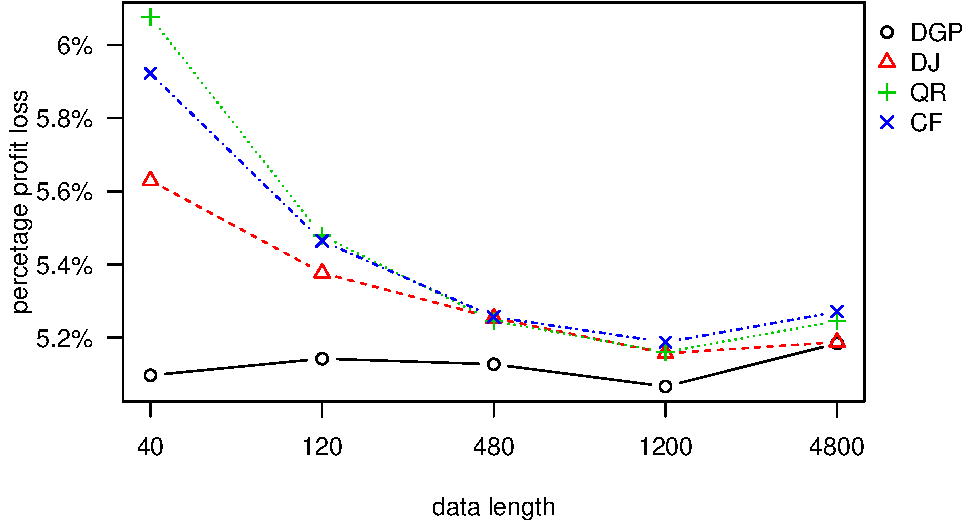
\includegraphics{linear-norm-plot_files/figure-latex/ppl0.3-1.pdf}
\caption{Percentage profit loss vs. data size at 0.3 target service level}
\label{fig:ppl0.3}
\end{figure}

In Figure \ref{fig:sl0.3}, every points represent the proportion of iterations that the demand is satisfied (e.g. 0.32 means the demand are satisfied in 6,400 of the 20,000 iterations). We can see that both the three methods and the DGP converge to the target service level 0.3 when data length grows. Yet, the disjoint method approaches the target service level from lower side while the proposed method and the quantile regression approach it from upper side. This phenomenon could be explained by the different mechanisms of the disjoint method and integrated method. The disjoint method forecasts the mean and variance of the demand distribution in the first phase. When the data size is small, the forecasted variance will be bigger than the true variance. Therefore, the solution of the optimal quantity in second phase will be 'far away' from 0.5, which leads to lower service level when data size is small. On the other hand, the integrated method approaches the true optimal quantity by applying the optimisation algorithm directly on total profit. Therefore, even if there are two quantity value that have equal distance from the optimal quantity, the algorithm will always favor the one with better profit. In this particular profit function, the algorithm will always favor the quantity leads to higher service level.

\begin{figure}[h]
\centering
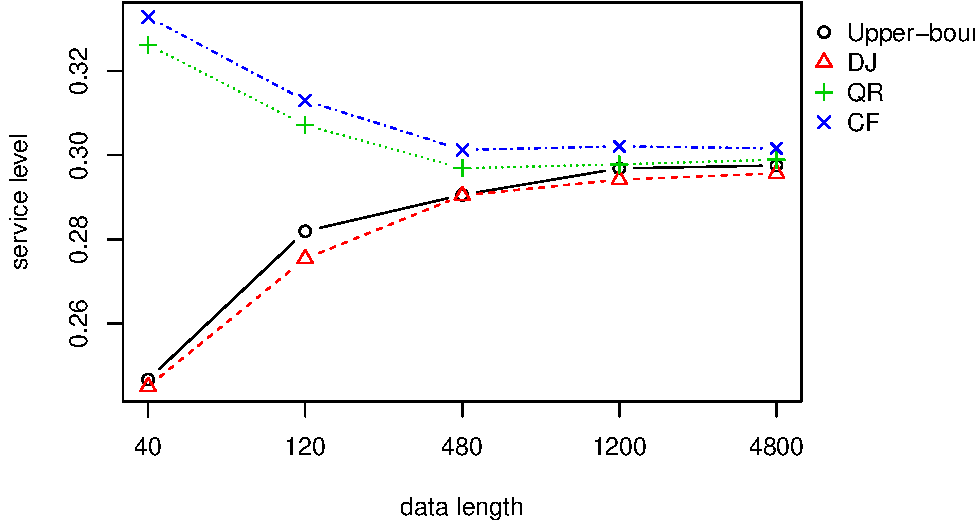
\includegraphics{linear-norm-plot_files/figure-latex/sl-3.pdf}
\caption{Service level vs. data size at 0.3 target service level}
\label{fig:sl0.3}
\end{figure}

By fixing the target service level, we can compare the performance of methods in different data size in Table \ref{tab:size_effect0.3}.

\begin{table}[h]
\caption{Size effect on percentage profit loss and service level at 0.3 target service level}
\label{tab:size_effect0.3}
\centering \resizebox{\linewidth}{!}{
\begin{tabular}[t]{ccccccccc}
\toprule
\multicolumn{1}{c}{\textbf{ }} & \multicolumn{4}{c}{\textbf{Percentage profit loss}} & \multicolumn{4}{c}{\textbf{Average service level}} & \multicolumn{4}{c}{\textbf{Fill rate}} \\
\cmidrule(l{3pt}r{3pt}){2-5} \cmidrule(l{3pt}r{3pt}){6-9} \cmidrule(l{3pt}r{3pt}){10-13}
Data size & DGP & disjoint & quantile & proposed & DGP & disjoint & quantile & proposed & DGP & disjoint & quantile & proposed\\
\midrule
40 & 5.10\% & 5.63\% & 6.08\% & 5.92\% & 0.247 & 0.245 & 0.326 & 0.333 & 89.53\% & 88.05\% & 90.04\% & 90.76\%\\
120 & 5.14\% & 5.38\% & 5.48\% & 5.46\% & 0.282 & 0.275 & 0.307 & 0.313 & 90.62\% & 89.68\% & 90.71\% & 91.04\%\\
480 & 5.13\% & 5.25\% & 5.25\% & 5.26\% & 0.291 & 0.290 & 0.297 & 0.301 & 90.92\% & 90.52\% & 90.87\% & 91.04\%\\
1200 & 5.07\% & 5.16\% & 5.16\% & 5.19\% & 0.297 & 0.294 & 0.298 & 0.302 & 91.06\% & 90.75\% & 90.97\% & 91.11\%\\
4800 & 5.18\% & 5.19\% & 5.25\% & 5.27\% & 0.298 & 0.296 & 0.299 & 0.302 & 90.96\% & 90.90\% & 90.90\% & 91.02\%\\
\bottomrule
\end{tabular}} 
\end{table}

On the other hand, we can also compare the methods' performance regarding to different target service levels while fix the data size in Table \ref{tab:level_effect40} and \ref{tab:level_effect4800}. When data size is big enough, as in Table \ref{tab:level_effect4800}, different target service level doesn't make too much effect on the performance of methods. However, it is worth noticing that when the data size is small, in Table \ref{tab:level_effect40}, the disjoint method performed very differently from other methods. 

\begin{table}[h]
\caption{Target service level effect on percentage profit loss and service level at 40 data size}
\label{tab:level_effect40}
\centering
\resizebox{\linewidth}{!}{
\begin{tabular}[t]{ccccccccc}
\toprule
\multicolumn{1}{c}{\textbf{ }} & \multicolumn{4}{c}{\textbf{Percentage profit loss}} & \multicolumn{4}{c}{\textbf{Average service level}} \\
\cmidrule(l{3pt}r{3pt}){2-5} \cmidrule(l{3pt}r{3pt}){6-9}
Target service level & DGP & disjoint & quantile & proposed & DGP & disjoint & quantile & proposed\\
\midrule
0.5 & 4.91\% & 5.35\% & 5.67\% & 5.51\% & 0.502 & 0.443 & 0.502 & 0.505\\
0.63 & 14.28\% & 15.25\% & 16.15\% & 15.62\% & 0.671 & 0.586 & 0.601 & 0.609\\
0.3 & 5.10\% & 5.63\% & 6.08\% & 5.92\% & 0.247 & 0.245 & 0.326 & 0.333\\
\bottomrule
\end{tabular}}
\end{table}

\begin{table}[h]
\caption{Target service level effect on percentage profit loss and service level at 4800 data size}
\label{tab:level_effect4800}
\centering
\resizebox{\linewidth}{!}{
\begin{tabular}[t]{ccccccccc}
\toprule
\multicolumn{1}{c}{\textbf{ }} & \multicolumn{4}{c}{\textbf{Percentage profit loss}} & \multicolumn{4}{c}{\textbf{Average service level}} \\
\cmidrule(l{3pt}r{3pt}){2-5} \cmidrule(l{3pt}r{3pt}){6-9}
Target service level & DGP & disjoint & quantile & proposed & DGP & disjoint & quantile & proposed\\
\midrule
0.5 & 4.92\% & 4.92\% & 4.96\% & 4.96\% & 0.492 & 0.492 & 0.493 & 0.494\\
0.63 & 14.02\% & 14.04\% & 14.22\% & 14.20\% & 0.626 & 0.626 & 0.626 & 0.624\\
0.3 & 5.18\% & 5.19\% & 5.25\% & 5.27\% & 0.298 & 0.296 & 0.299 & 0.302\\
\bottomrule
\end{tabular}}
\end{table}

\subsection{Nonlinear profit function}
In this subsection, we consider the simulation where, as before, the error term of the demand follows normal distribution, and we know the model of the data generating process, but the underlying profit function is nonlinear\footnote{$
        \pi(Q,y)=
        \begin{cases}
            20y-8Q-4(Q-y)+5\E[\min \{(Q-y),u\}],& \text{if } Q\geq y\\
            20Q-8Q-7(y-Q)^2,& \text{if } Q< y,
        \end{cases}$ and $u\sim \mathcal{U}(0,50)$} (solution see \cite{KK18}). 
In this experiment, we pay specific attention to the percentage profit loss, and we explore how the performance changes on both the proposed method and the disjoint method when we alter the profit function to nonlinear. The data will still be generated from ARIMA process, and the five data lengths are maintained. The results can be seen in 

%%%%%%%%%%%%%%%%%%%%%%%%%%%%%%
\section{Concluding Remarks} \label{se:end}

BLAH...

%%%%%%%%%%%%%%%%%%%%%%%%%%%%%%
\printbibliography

%%%%%%%%%%%%%%%%%%%%%%%%%%%%%%
\newpage
\begin{center}
{\bf\Large Appendices}
\end{center}

\appendix





\section{Derivation of quantile regression transformation}\label{app:A}
We have:
\[
    \min[a,b]=a-[a-b]^+,
\]
and
\[
    a-b=[a-b]^+-[b-a]^+.
\]
We can transform:
\[
    \begin{aligned}
        \pi(\mathbf{x}_t^{\mathsf{T}}\boldsymbol{\beta},y_t)
        &=p\min[\mathbf{x}_t^{\mathsf{T}}\boldsymbol{\beta},y_t]-v\mathbf{x}_t^{\mathsf{T}}\boldsymbol{\beta}+c_h[\mathbf{x}_t^{\mathsf{T}}\boldsymbol{\beta}-y_t]^++c_s[y_t-\mathbf{x}_t^{\mathsf{T}}\boldsymbol{\beta}]^+\\
        &=p\{\mathbf{x}_t^{\mathsf{T}}\boldsymbol{\beta}-[\mathbf{x}_t^{\mathsf{T}}\boldsymbol{\beta}-y_t]^+\}-v\mathbf{x}_t^{\mathsf{T}}\boldsymbol{\beta}+c_h[\mathbf{x}_t^{\mathsf{T}}\boldsymbol{\beta}-y_t]^++c_s[y_t-\mathbf{x}_t^{\mathsf{T}}\boldsymbol{\beta}]^+\\
        &=(p-v)\mathbf{x}_t^{\mathsf{T}}\boldsymbol{\beta}+(c_h-p)[\mathbf{x}_t^{\mathsf{T}}\boldsymbol{\beta}-y_t]^++c_s[y_t-\mathbf{x}_t^{\mathsf{T}}\boldsymbol{\beta}]^+.
    \end{aligned}
\]
Therefore, we have (since $y_t$ is fixed):
\[
    \begin{aligned}
        &\text{max}\displaystyle\sum_{s=1}^t{\pi(\mathbf{x}_t^{\mathsf{T}}\boldsymbol{\beta},y_t)}\\
        &\quad=\text{max}\displaystyle\sum_{t=1}^s\{(p-v)\mathbf{x}_t^{\mathsf{T}}\boldsymbol{\beta}+(c_h-p)[\mathbf{x}_t^{\mathsf{T}}\boldsymbol{\beta}-y_t]^++c_s[y_t-\mathbf{x}_t^{\mathsf{T}}\boldsymbol{\beta}]^+\}\\
        &\quad=\text{max}\displaystyle\sum_{t=1}^s\{(p-v)[\mathbf{x}_t^{\mathsf{T}}\boldsymbol{\beta}-y_t]+(c_h-p)[\mathbf{x}_t^{\mathsf{T}}\boldsymbol{\beta}-y_t]^++c_s[y_t-\mathbf{x}_t^{\mathsf{T}}\boldsymbol{\beta}]^+\}\\
        &\quad=\text{max}\displaystyle\sum_{t=1}^s\{(p-v)[\mathbf{x}_t^{\mathsf{T}}\boldsymbol{\beta}-y_t]^+-(p-v)[y_t-\mathbf{x}_t^{\mathsf{T}}\boldsymbol{\beta}]^+\\
        &\qquad+(c_h-p)[\mathbf{x}_t^{\mathsf{T}}\boldsymbol{\beta}-y_t]^++c_s[y_t-\mathbf{x}_t^{\mathsf{T}}\boldsymbol{\beta}]^+\}\\
        &\quad=\text{min}\displaystyle\sum_{t=1}^s\{(v-c_h)[\mathbf{x}_t^{\mathsf{T}}\boldsymbol{\beta}-y_t]^++(p-v-c_s)[y_t-\mathbf{x}_t^{\mathsf{T}}\boldsymbol{\beta}]^+\}
    \end{aligned}
\]

\section{Derivation of scale and shift equivalence}\label{app:B}
Scale equivalence:
\[
    \begin{aligned}
        \hat{\boldsymbol{\beta}}(a\mathbf{y},\mathbf{X})
        &=\text{argmax}_{\boldsymbol{\beta}\in \mathbb{R}^{p+1}}\displaystyle\sum_{t=1}^s{\pi(\mathbf{x}_t^{\mathsf{T}}\boldsymbol{\beta},ay_t)}\\
        &=\text{argmin}_{\boldsymbol{\beta}\in \mathbb{R}^{p+1}}\displaystyle\sum_{t=1}^s{\{c_o[\mathbf{x}_t^{\mathsf{T}}\boldsymbol{\beta}-ay_t]^{+}+c_u[ay_t-\mathbf{x}_t^{\mathsf{T}}\boldsymbol{\beta}]^{+}\}}\\
        &=\text{argmax}_{\boldsymbol{\beta}\in \mathbb{R}^{p+1}}\displaystyle\sum_{t=1}^s{\pi\left(\mathbf{x}_t^{\mathsf{T}}\frac{\boldsymbol{\beta}}{a},y_t\right)}\\
        &=a\hat{\boldsymbol{\beta}}(\mathbf{y},\mathbf{X}).
    \end{aligned}
\]
    
Shift equivalence:
\[
    \begin{aligned}
        &\hat{\boldsymbol{\beta}}(\mathbf{y}+\mathbf{X}\gamma,\mathbf{X})\\
        &\quad=\text{argmax}_{\boldsymbol{\beta}\in \mathbb{R}^{p+1}}\displaystyle\sum_{t=1}^s{\pi(\mathbf{x}_t^{\mathsf{T}}\boldsymbol{\beta},y_t+\mathbf{x}_t^{\mathsf{T}}\gamma)}\\
        &\quad=\text{argmin}_{\boldsymbol{\beta}\in \mathbb{R}^{p+1}}\displaystyle\sum_{t=1}^s{\{c_o[\mathbf{x}_t^{\mathsf{T}}\boldsymbol{\beta}-y_t-\mathbf{x}_t^{\mathsf{T}}\gamma]^{+}+c_u[y_t+\mathbf{x}_t^{\mathsf{T}}\gamma-\mathbf{x}_t^{\mathsf{T}}\boldsymbol{\beta}]^{+}\}}\\
        &\quad=\text{argmax}_{\boldsymbol{\beta}\in \mathbb{R}^{p+1}}\displaystyle\sum_{t=1}^s{\pi[\mathbf{x}_t^{\mathsf{T}}(\boldsymbol{\beta}-\gamma),y_t]}\\
        &\quad=\hat{\boldsymbol{\beta}}(\mathbf{y},\mathbf{X})+\gamma.
    \end{aligned}
\]


\end{document}